\documentclass[12pt, a4paper]{article}

\usepackage{statprojekt}
\newcommand{\naslov}{Projektna naloga iz Statistike}

\begin{document}

\renewcommand{\headheight}{20pt}

\date{September 2024}
\maketitle
\thispagestyle{empty}

\newpage

\section{Kibergrad}

Preučujemo dohodke družin v mestu Kibergrad. Imamo informacije o $43.886$ družinah, 
ki živijo v eni od štirih četrti: v severni četrti stanuje $10.149$ družin, v
vzhodni $10.390$, v južni $13.457$ in v zahodni $9.890$. Pomagamo si 
s programom \texttt{kibergrad.py}.

Iz vsake četrti vzemimo enostavni slučajni vzorec velikosti $100$. 
Dohodke lahko primerjamo s pomočjo vzporednih škatel z brki, ki 
so prikazane na sliki \ref{img:cetrti}.
\begin{figure}[H]
    \centering
    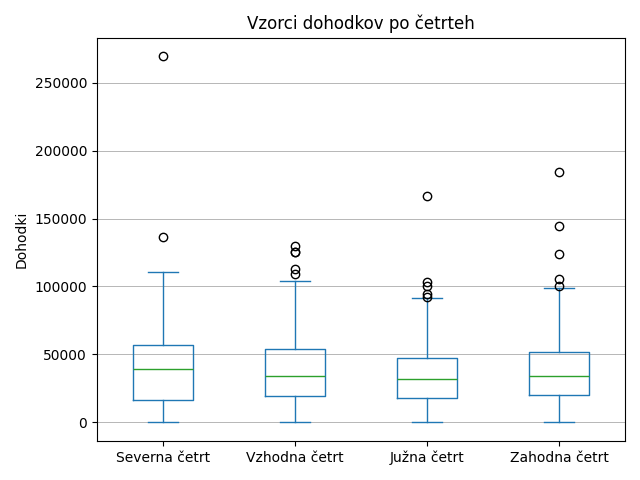
\includegraphics[width=12cm]{vse_cetrti.png}
    \caption{Škatle z brki za dohodke posamezne četrti.}
    \label{img:cetrti}
\end{figure}
Najprej opazimo, da je v severni četrti osamelec, ki močna izstopa. Prav tako so maksimum, tretji 
kvartil in mediana v severni četrti največji, vendar razlika ni dovolj velika, 
da bi lahko pri tako majhnem vzorcu sklepali, da so dohodki severne četrti 
najvišji. Zdi pa se, da so dohodki severne četrti malenkost višji kot dohodki 
južne četrti, pri kateri so vse prej omenjene vrednosti najmanjše. 

Zdi se, da v splošnem četrt ne vpliva močno na velikost dohodka.


Sedaj vzemimo še štiri enostavne slučajne vzorce velikosti $100$ 
iz severne četrti in poglejmo vzporedne škatle z brki za vzorce
iz severne četrti. Prikazane so na sliki \ref{img:sever}.
\begin{figure}[H]
    \centering
    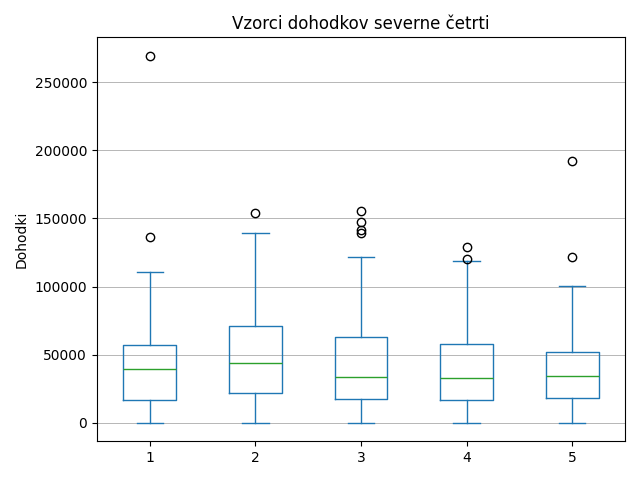
\includegraphics[width=12cm]{sever.png}
    \caption{Škatle z brki dohodkov severne četrti.}
    \label{img:sever}
\end{figure}
Vse mediane so večje od $33.000$, njihovo povprečje je približno 
$36.500$. Zdi se, da lahko s precejšnjo sigurnostjo sklepamo, da je večina 
dohodkov višjih od $33.000$.

V novih vzorcih ne opazimo tako ekstremnih osamelcev kot pri prvem vzorcu. Večina 
osamelcev ni zelo oddaljenih od maksimuma.

Za konec si poglejmo še varianco dohodka pojasnjeno s četrtmi in preostalo
(rezidualno) varianco. Naj bo $N$ velikost populacije, $N_i$ velikost 
populacije $i$-te četrti in $w_i$ velikostni delež $i$-te četrti. Naj bo
$\mu$ povprečni dogodek in $\sigma^2$ varianca dohodka Kibergrada,
$\mu_i$ in $\sigma_i^2$ pa zaporedoma povprečni dohodek in varianca 
dohodka $i$-te četrti. Pojasnjena in nepojasnjena varianca sta zaporedoma 
določeni s formulama
\[
    \sigma^2_B := \sum_{i=1}^{4} w_i(\mu_i - \mu)
    \quad \text{in} \quad
    \sigma^2_W := \sum_{i=1}^{4} w_i\sigma_i^2.
\]
Izračunamo, da je 
\[
    \sigma^2_B = 9.252.923
    \quad \text{in} \quad
    \sigma^2_W = 1.017.226.451.
\]
S četrti pojasnjeni 
standardni odklon je torej $3.042$. Povprečni dohodki četrti, 
so enaki $45.759$, $41.235$, $37.473$ in $42.158$, torej je 
standardni odklon v primerjavi z njimi majhen. To se ujema z 
opažanjem, da četrt ne vpliva močno na velikost dohodka.
\newpage

\section{Lomljivost najlonskih palic}
Na vzorcu $280$ najlonskih palic preizkušamo njihovo lomljivost. Rezultati 
preizkusa so prikazani v tabeli \ref{table:lomljivost}. Pri analizi 
si pomagamo s programom $\texttt{najlonske\_palice.py}$.
\begin{table}[H]
    \centering
    \begin{tabular}{|l||l|l|l|l|l|l|}
        \hline
        št.~lomov & 0   & 1  & 2  & 3  & 4 & 5 \\ \hline
        št.~palic & 157 & 69 & 35 & 17 & 1 & 1 \\ \hline
    \end{tabular}
    \caption{Rezultati preizkusa lomljivosti.}
    \label{table:lomljivost}
\end{table}
Privzemimo, da je število mest, na katerih se je palica 
zlomila porazdeljeno binomsko $\Bin(5, p)$ za določen neznan $p$.
Privzemimo tudi, da so palice med seboj neodvisne.

Pri teh predpostavkah je logaritem verjetja podan z
\[
    l(p, x) = \log\prod_{i=1}^n \binom{280}{x_i}p^{x_i}(1-p)^{5-x_i}.
\]
Izračunamo, da je maksimum 
dosežen pri približno $p = 0{,}1421438163551369$. Ta vrednost
nam predstavlja oceno $p$ po metodi največjega verjetja.


\end{document}